%!TeX encoding = UTF-8

%%%%%%%%%%%%%%%%%
% 不能在文章中使用中文
% 模板文档: http://mirror.aut.ac.nz/CTAN/macros/latex/contrib/apa6/apa6.pdf
% \section{我是一级标题} 一级标题
% \subsection{我是二级标题} 二级标题
% \subsubsection{我是三级标题} 三级标题
% 带括号引用 \parencite{文章简写}
%%%%%%%%%%%%%%%%%

%%%%%%%%%%%%%%%%%
% 文档定义
%%%%%%%%%%%%%%%%%
\documentclass[a4paper]{article}
\usepackage[american]{babel}
\usepackage{csquotes}
\usepackage[style=apa,sortcites=true,sorting=nyt,backend=biber]{biblatex}
% 其他包
% 数学符号
\usepackage{amssymb}
% 导入csv表格
\usepackage{csvsimple}
% 导入图片
\usepackage{graphicx}
\graphicspath{ {./images/} }
% 超链接支持
\usepackage[hidelinks]{hyperref}
% 多行注释
\usepackage{verbatim}
% 插图caption
\usepackage{caption}
\usepackage{subcaption}
% 缩放table
\usepackage{adjustbox}
\DeclareLanguageMapping{american}{american-apa}
% \addbibresource{bibliography.bib}

\title{An IT Deployment Plan for Department of Computing of Ara Institute of Canterbury}
\usepackage{fancyhdr}
\pagestyle{fancy}
\lhead{Lu \& Wei}
\chead{BCIS301-A2}
% 页眉中的标题
% \shorttitle{}

% 作者/组织
% \twoauthors{Louis Lu}{Zhong Wei}
\author{
  Louis Lu
  \and
  Zhong Wei
}
% \twoaffiliations{Ara Institute of Canterbury}{Ara Institute of Canterbury}

% \leftheader{}

% \abstract{}
% \keywords{}

%%%%%%%%%%%%%%%%%
% 文档正文
%%%%%%%%%%%%%%%%%
\begin{document}
% 隐藏页眉
% \thispagestyle{otherpage}
% 标题
\maketitle

%%%%%%%%%%%%%%%%%
% 目录
%%%%%%%%%%%%%%%%%
\clearpage
\tableofcontents
\clearpage

%!TEX root = ../assignment2.tex


\section{Introduction}

In this article, we seek to develop the 3-year IT deployment Plan for the Department of Computing of Ara Institute of Canterbury.

\subsection{Background}
% Ara 学校 介绍
Ara Institute of Canterbury is the biggest vocational training institute, which provides world-class, tertiary-level education throughout the Canterbury and Waitaki region. It provides 254 qualifications according to the New Zealand Qualification Authority(NZQA).

% Computing Department 介绍
Department of Computing is one of the departments, dedicated to information, communication and technology. The department offers various programs targeting programming, networking and information system.


\subsection{The Goal of the Deployment Plan}
% 提出 3 年 goal
Given the background of the department and the institute, the article seeks to produce a 3-year IT deployment plan with the ultimate goal of "teach better, study better".


\subsection{Topics and Structure}
To achieve the goal, research is conducted by interviews with staff, analysis of interview, proposals of solutions, evaluation of proposals, building the hierarchy of deployment plan.

To express the research in an organized way, the following structure is built to further all the topics.

In the introduction section, a general introduction is given, which covers the description of the institution, the department and how the article tries to research.

In methodology, the procedures of researching steps are defined, which covers how the data collected, how the analysis on data is conducted, how the potential solutions are made, how the solutions are evaluated, and eventually how the complete hierarchy of planning is delivered.

In data analysis, the comprehensive analysis is illustrated with the aforementioned method in the previous section. Sub-topics are given and issues are listed with detailed samples in each sub-topic. Then, one of the generic IT deployment strategies is chosen which fits the organization among 6 general types. The strategy chosen will be one factor for the proposals of solutions in the next section.

In solution analysis, proposals of solutions are offered coherently and cohesively to each sub-topic in the previous sections accordingly. An evaluation defined in the methodology is conducted for selecting the best solutions that benefit the organization.

In the deployment plan, a hierarchically structured deployment plan is delivered, which includes all the building elements in the relevant sections above.

Finally, a summary is given to conclude the result of this article.
% % 总起
% In this article, we seek to identify critical success factors for IT projects by literature review, and then try to build an evaluation system to make an IT project successful. With that aim, we conduct a qualitative analysis to gather all the significant points of what the literature argue regarding this topic. A quantitative model is set up to select and prioritize the findings. The outcome of the model is a solution list. The aforementioned process will be done twice with respective resources, which results in an evaluation tool for researchers and practitioners to avoid similar failures in IT projects.

% % 背景
% \subsection{Background}
% IT projects today tend to be agile, technical and complex\parencite[p. 2]{4} where pitfalls, issues and risks are everywhere in terms of time, people and budget. From a
% project management perspective, the project was 193\% over schedule, 419\% over budget, and 130\% over scope\parencite[p. 8]{6}. A shockingly high failure rate also can be seen across some other publications in literature\parencite{2,3}.

% % 背景中的三个关键词
% \subsection{Keywords}
% We investigate the literature and zoom in with the following keywords that influence success or failure of an IT project the most, which are project management, change management and risk management.

% \paragraph{Project Management}
% Project management is the planning to deliver the deliverables in a project, which academia believes, consists of 4-phase planning: initiating, planning, executing and controlling, while some researchers introduce the idea that this deliverable-targeted plan is considered as initiation, contagion, control and integration when a specific model in ERP projects is built\parencite[p. 3]{2}. Project management covers a lot of sub-areas such as time, scope, budget, quality, issues, risk and change. Success will be presented when a sophisticated project manager arrange them well in every stage.

% \paragraph{Change Management}
% Change management, as mentioned previously, is a sub-component of project management which researchers\parencite{3,6} have been putting emphasis on. In such an agile and technical and complex industry, the complexity of a project has inevitably made decision makers implement some changes for all or some stakeholders to transit to another new system\parencite[p. 1]{3} so that a better quality of the deliverables will be produced with the three constraints: scope, time, budget. The idea of change management has been regarded as a progressive method for attaining strong-minded conversion within a business or individuals sometimes\parencite[p. 3]{3}.

% \paragraph{Risk Management}
% Despite the fact that risk management is yet another sub-component of project management, a recent research by Bunker enlightens us by introducing disaster management from a change management perspective instead of a traditional project management perspective\parencite[p. 10]{6}. Intriguingly and similarly, the idea of emergent and scenario driven disaster management can be applied to the risk management.

% % 文章结构
% \subsection{Structure}
% The article is divided into 7 sections: introduction, methodology, findings of Phase 1, findings of Phase 2, conclusion, summary and reflections. In introduction, a brief information is given, stating what we are investigating and what result we will produce. 3 aforementioned keywords are also introduced for future reference. The methodology describes how we conduct our research. A subsequent findings of Phase 1 will be presented with details using the defined method with data, where an evaluation is done. The findings of Phase 2 is structurally similar to the previous section, but with 10 case studies. In outcome, we will compare and contrast findings of both phases, then try to make an evaluation tool from our findings. The conclusion will revisit what we will have covered in previous sections. Summary will be provided as a briefing of the whole article. And eventually, there is a reflections section discussing the values and limitations of this research.

%!TEX root = ../assignment2.tex

\section{Methodology}

\subsection{Synopsis}

For the deployment plan, research is conducted to build this plan with the following steps.

First, data is collected by both the transcripts of existing interviews and the transcripts that the authors have compiled with working staffs of the Computing Department.

Next, with all the data prepared, data analysis is done by first investigating the functions inside the organization, also known as thematic analysis, then by a qualitative analysis which identifies the facts and issues. To better find possible solutions in this context, a generic IT deployment strategy is selected among the options.

With the issues identified and the best-fit generic IT deployment strategy, solutions are proposed for each function of the organization. Then, a framework is utilized to select the best solutions among all the proposals.

Finally, a hierarchy of the deployment plan is illustrated by filling the results above into the tree structure, which visually present the deployment plan.


\subsection{Data Collection}	
	% 采访稿
The data consists of two sources. The first source is the existing transcripts of interviews conducted by former students, in which 6 staff members are interviewed, giving responsibilities, reflecting the structural layout of the department and commenting on the existing issues. The transcripts cover the following topics of Cisco network academy, ethics, operation manager, software engineering and TechLabs.
	% 对 Sarah Medhi的采访
The second source is from our interviews of the acting head of the department and a student and teaching assistant. The interviews are held in two sessions and questions are raised about issues and opinions on the department.

\subsection{Data Analysis}
With all the transcripts of interviews compiled, data analysis commences with the following steps. 
	% function analysis (thematic analysis)
Functions are first identified by thematic analysis. The current situation and technologies are investigated in the thematic analysis, which serves as the assets for the next step to be illustrated next. The functional analysis covers the current jobs and duties inside the department and the related IT technologies deployed in the department.
	% qualitative analysis

With all the functions inside the department defined, a qualitative analysis is progressed, trying to find all the issues that can be classified into primary themes after collecting their secondary themes based on facts. In other words, the outcome of qualitative analysis are facts, issues, secondary themes, and primary themes.

	% Generic IT Deployment Strategies (centrally planned)
Generic IT deployment strategies conclude the general rules applied to a variety of organization. There are 7 types of organizations: centrally planned, leading edge, free market, monopoly, scarce resource, and a necessary evil. A type is selected to draft solutions and to select the solutions, according to the features that the Computing Department has.

\subsection{Solution Analysis}
	% 对每一类问题给解决方案
Solutions are given to each primary theme, the generalized topics are identified in the qualitative analysis. All the potential solutions are the candidates that will be evaluated in a framework to select the best practice to be done.
	% 得分表算法
The Evaluation framework tries to assess the ability to solve the generalized topics of primary themes in qualitative analysis. For each solution, the score calculates as follows.

$$
R_{S_i} = \sum_{j=1}^n{r_{S_i, t_j}}
$$

$R$ denotes a final rating. $S_i$ is a candidate solution. Thus, $r_{S_i}$ is the final rating of a given candidate solution. $t_j$ is the primary theme of a given generalized issue. Therefore, $\sum_{j=1}^n{r_{S_i, t_j}}$ is a rating out of 10 for the ability to solve the specific generalized topic of issues $S_{t_i}$. If the solution brings positive impact of the given topic of issues, a positive score will be rated. On the contrary, a negative score will be marked if there is a negative effect on the same topic of issues. The range of the score $R_{Si_{t_j}} \in [-10, 10]$

The average score of $\bar{R_{S}}$ of all the solutions are calculated. Every solution above the average score is considered as approved solution to be selected the deployment plan.


\subsection{Deployment Plan}
	% 对evaluated 的方案放入hierachy
The deployment plan puts all the building blocks into a hierarchy structure to illustrate the whole decision-making process in a visually expressive way, where the goals, issues, solutions, the selected of solutions and the connections between the elements.


% % 总流程
% \subsection{Synopsis}
% The study consists of two phases. For each phase, a qualitative analysis is first carried out, identifying all the gaps and possible solutions(proposals) that the researchers suggest regarding success, failure, and risks in ICT projects. To identify these themes, a list of excerpts(facts) is built and then reworded as proposals. Those proposals are evaluated in a quantitative model which results in a solution list for each phase. The items in both solution lists are compared and contrasted and reshaped into a mark sheet as the evaluation tool we create. Additionally, Tags, such as affected phases and affected roles, are used for the evaluation process; the primary themes in qualitative analysis are top-level categories in the final outcome of the evaluation tool we create. Following paragraphs will give more details about how the tags are utilized throughout the research method.


% % 列举文章和主题
% \subsection{Selection of Literature}
% In Phase 1, we focus on three themes regarding the success of an IT project, namely project management, change management, and risk management. Also, CSF(critical success factor), CFF(critical failure factor), ERP(enterprise resource planning) are the keywords used in the literature selections. All the sources should be from professional journals and forums published within 10 years from now, around 10 pages of length and referenced by other researchers, which reliability and professionalism can be assured.

% In Phase 2, we are given 10 case studies in \citetitle{case_study} which illustrates 10 IT deployment projects in Victoria, Australia. We conduct our research using the same procedure as in Phase 1.

% % 如何 coding
% \subsection{Data Analysis}
% When utilizing the aforementioned selection of literature for qualitative analysis, we seek to identify issues, solutions and/or conclusions that authors have deduced or based on. Excerpts of facts are compiled in this stage. Furthermore, the phases and the roles of stakeholders involved are also noted when a possible clue is identified. Priority information in the same research context is recorded as well, which as known weights. For each of the excerpt, we reword the statement as possible proposals. All possible proposals are also tagged with affected phases and affected roles from their respective excerpt. This asset is now ready for the subsequent evaluation processes.

% % 如何做 evaluation framework
% \subsection{Evaluation Process}
% With this captured data in each phase, an evaluation is designed where all the proposals are listed and evaluated by how a given proposal affects on the phases of a project and on the roles of stakeholders in corresponding phases. To better employ the prioritized proposals by some researchers who use statistical models, a cross-contextual coefficient is introduced during the evaluation process. In the evaluation process, global influence score of a proposal in a specific research context is calculated by the following formula \ref{brief}.
% \begin{equation}
% g_{C_{i},j} = \mathit{k_{C_{i},j}}l_{C_{i},j},\ C_{i,j} \in C_{i},\ C_{i} \in \mathbb{C}
% \label{brief}
% \end{equation}

% In formula \ref{brief}, $\mathbb{C}$ denotes the set of all research contexts. And for each research context $C_{i}$ which is an element in $\mathbb{C}$, $C_{i,j}$ denotes a proposal in the given research context $C_{i}$. $g_{Ci,j}$ is the global influence score of a proposal in a given research context $C_{i}$. Similarly, $l_{C_{i},j}$ is the local influence score of the same proposal; $\mathit{k_{C_{i},j}}$ is the cross-contextual coefficient for the same proposal. Each element on the right hand side of formula \ref{brief} can be calculated respectively as follows.
% \begin{equation}
% \mathit{k_{C_{i},j}} = \frac{f_{C_{i,j}}}{\bar{f_{C_i}}}
% \label{coefficient}
% \end{equation}
% \begin{equation}
% \bar{f_{C_i}} = \frac{1}{n}\left (\sum_{m=1}^n{f_{C_{i,m}}}\right)
% \label{mean}
% \end{equation}
% \begin{equation}
% l_{C_{i},j} = |P_{C_{i,j}}||R_{C_{i,j}}|
% \label{local_influence}
% \end{equation}

% In formula \ref{coefficient} and \ref{mean}, $f_{C_{i,j}}$ denotes the local influence score in a research context $C_{i}$ and $\bar{f_{C_i}}$ is the arithmetic mean value of all local influence scores of proposals in a given context $C_{i}$.

% In formula \ref{local_influence}, $l_{C_{i},j}$ is the local influence score of a given proposal $C_{i,j}$. $|X|$ denotes the cardinality of the given set $X$. $P_{C_{i,j}}$ is the set of affected phases by the proposal $C_{i,j}$. Similarly, $R_{C_{i,j}}$ is that of affected roles of stakeholders in the same context.

% Thus, the global influence score of a given proposal that denotes as $g_{C_{i},j}$ can be calculated as follows:
% \begin{equation}
% g_{C_{i},j} =
% \frac
% % 分子 k local=(P R)
% {f_{C_{i,j}} |P_{C_{i,j}}| |R_{C_{i,j}}|} 
% % ----分式线-----
% % 分母 f平均
% {\frac{1}{n}\left (\sum_{m=1}^n{f_{C_{i,m}}}\right)}
% % 满足条件
% ,\ 
% C_{i,j} \in C_{i},\ C_{i} \in \mathbb{C}
% \label{final}
% \end{equation}

% A higher score of $g_{C_{i},j}$ indicates that the proposal has a wider and deeper influence on project success. We post-process the result of a score by descending ranking, in which we select the ones higher than average value. This subset of proposals are tagged by sub-topics and enrolled in the solution checklist.

% \subsection{Making of Evaluation Tool}
% \label{section:tool}

% First, there is a comparison and contrast of the solutions of both phases to evaluate the agreement between the phases.

% If there is some degree of agreement that can contribute to the evaluation tool, a 2-level hierarchical structure mark sheet will be created using the following method.

% The 2-level hierarchical mark sheet consists of an outer level of the primary themes we used in our entire research; and the inner level of the sub-themes of when the solution is recommended with a new round of qualitative analysis. The solutions are all populated under the sub-themes with normalized weights calculated as follows.
% \begin{equation}
% w_i = \frac{100s_i}{\sum_{i=1}^n{s_i}}\%, s_i \in \mathbb{S}
% \label{formula:toolweight}
% \end{equation}

% In formula \ref{formula:toolweight}, $\mathbb{S}$ denotes the collection of solutions of both phases. $s_i$ is a solution in same collection. $w_i$ is the weight of a given solution $s_i$. $g_i$ is the global influence score of the same given solution.


% When a user mark a project with the mark sheet, the user rate out of 10, on how well the project has done given a solution. The scores are calculated as follows.
% \begin{equation}
% s_i = \frac{r_i}{10w_i\%}, S = \sum_{i=1}^n{s_i}
% \label{formula:toolscore}
% \end{equation}
% In formula \ref{formula:toolscore}, $S$ denotes the final score. $s_i$ is the score of a given solution, $w_i$ is the weight of the same solution, $r_i$ is the user rating out of 10.

% A higher final score of $S$ indicates the higher possibility of success.

%!TEX root = ../assignment2.tex

\section{Data Analysis}

\subsection{Overview of Data}
% In our selection of literature, 6 articles are employed. \citetitle{1} and \citetitle{2} are on project management. \citetitle{3} argues about change management while \citetitle{4} and \citetitle{5} are on risk management. \citetitle{6} gives an overview and an update of information system success and failure, which is composed by an affiliation of famous scholars in the field.
Besides the interview scripts notes which was taken by Sarah last year, we also interviewed Sarah and Mehdi two weeks ago. Though Dabid is also planned to be interviewed by us, finally we didn't get a chance to interview him for unknown reasons. So those scripts and both interview to Sarah and Mehdi comprised our information resources. Based on this information, we conducted a qualitative analysis and got thirty-two facts across twelve functions.

\subsection{Primary Themes}
Five primary themes of the issues were finally identified from thirty-one secondary themes in our coding data, which were budget, communication, manual process, security, and software. 

\subsubsection{Budget} is about the expenditure for a department in annual reckoning. It is usually fixed but deficient since unexpected expense happened casually. Insufficient budget was noticed through the research at the first phase . The interviewee from CISCO Network Academy informed us that they need more expensive switches and routers to extend the network being used. They need more space to accommodate student and equipments. They also want to attract more students to learn networking, and they need more money to carry out marketing activities. They actually met difficulties in convincing Ara that paying more money to Cisco Network Academy is worthy enough. Budget issue is a realistic problem, while it is mainly a governance problem. Mostly, we cannot resolve it by technical means.

\subsubsection{Communication} has been recognized as a general issue for CISCO Network Academy and the Operations Manager. According the interview to the tutor of CISCO Network Academy, the desire to maintain a better connection with previous students was expressed. He also pointed out that nothing was taught on teaching students how to create connections with industry except the "geeky stuff" in their Academy. For our students, it is important to own soft power besides their technical power to get competitive power in the talents market. How to create a safe and effective social community? It is one of the important issue to be resolved. The Operation Manager claimed that "no one know we are the biggest CISCO system trainer in New Zealand". In Regards to the roles and responsibilities, there is a serious issue of lack of awareness and communication. Besides this complain, the engagment with student was also defective, it needs to be improved by better communication tool and mechanics.

\subsubsection{Manual process} is one of the most complained issue in this analysis. It was reported by almost all the interviewee, that is Mehdi, Sarah, the tutor from Ethics, the tutor from Tech Labs, the tutor from software engineering, the OP Manager. All of them have met some inconvenience from manual process in their daily work. Below are the details of these inconvenience.

\paragraph{Timetabling} The interviewee which is the OP manager claimed that there is no specific IT program for timetabling, she has to talk with individual tutors and manually find out which teaching sessions or hours are required, and manually put this information into a spreadsheet. Even more distressing is that this is not the end. Once she complete the task on the spreadsheet,she has to manually put the timetable data into tribal software. She is tired with these things, it is not only boring, inefficient, but also error-prone. 

\paragraph{CAPEX Requests} Similar scene occurs on processing CAPEX requests. The same OP Manager is also in charge of processing CAPEX requests for computing team. Mannually filling in forms is required. Manually tracking the status of each CAPEX requests is an impossible task. Thus, there is no way to guarantee if the money has been correctly spent. 

\paragraph{Result System} In regards to the results of the students, once a tutor confirmed the result for certain student, he or she could immediately get his or her result. It is good. However, in case the tutor makes a mistake with certain result, the tutor has to perform a manual process to change the result.  

Ethics	"Applications:
Have to fill out a form with aim and objectives"
Ethics	"Electronic versions of the completed form are sent to the committee

- Results Meeting:
     Used to identify students that may need additional Support
     Check consistency of grading
     Not a formal cross-checking process
     Preparation for the results meeting:
       No auto extraction from the Tribal Database
       Results are manually populated into a spreadsheet
       This spreadsheet is then discussed at the results meeting
       Occurs at the end of every semester prior to results being confirmed as final"
OP Manager	"Re-Enrolment – System generated form that is required to be printed and signed by staff/students
- All manual with forms – no System
   Would like for it to be more automated"
OP Manager	"Change management processes within the department have not been going well due to lack of resources
  - Groups of lecturers from every group get together to formally discuss and evaluate new curses
      Forms need to be filled out
      All paper based/MS word
      No application used to simplify the process
  - Institution doesn’t require lecturers to re-evaluate courses, but most do anyway
      Not a formal process
      Each program has a MOE required review
      Not at a course level, but at a program level (IE degree)
  - Academic services assist with the documentation side of things
      Not assisted by an IT system"
OP Manager	"Moderation of assessments
  - Decided to have a 5 year strategy
  - Each 5 yrs each course has an external assessment
  - Priority is given to new courses/tutors
  - Completely manual process
  - All in a spreadsheet
  - Someone has to remember to do it
  - Manual follow up if this has been done
  - Would like to try and minimalise reliance on actual people 
      Risk reduction
      Tech could assist"
Software Engineering Tutor	"Important to do a register for each class
  - Either pass a sign in sheet around, or update on tribal
  - Tried to do it all automatically
      Attendance database is run by tribal
      Don’t allow an automatic batch update
  - Tried RFID card scanning
      Project completed and worked well
        Can’t be updated into tribal
  - Originally just got students to write their names on paper
      Too hard to pick out names
  - Looked at facial recognition
      Already have pictures on files from student ID
      Would need permission from students to film the class
      Would still need to manually update TRINBAL
  - Gave up and now uses a printed name list, with students signing by their name
      Easier to recognise names
      Hard as a non-native English speaker to read handwriting"
Tech Labs Tutor	"Stuff is bought through the IT department
- Time consuming
- Lots of paperwork
- Forms hard/not liked
- Rather go out and buy an item then charge it back"
Sarah	Booking a room needs to talk to Sandy 
Sarah	Fill timesheet to get paid.
Mehdi	"-	The internal process is manual
-	Change something in course (eg. network protocol)
-	Form -> Division -> Approval
-	Should be inspected by two people to approve
-	Manual monitoring"

% \paragraph{Structure} means the structure of an organization.
\paragraph{Security} is ...


\paragraph{Software} is ...

\subsection{Gaps and Solutions}

% 这里加个层级图 ? 就是一堆问题(1层),一堆解决方案(2层), 选定的解决方案(3层),
% The gaps and the solutions often express the same meanings but with different wording. Gaps are often stated as "lack of something" while the solutions suggest to supplement the missing part. Therefore, we only collect the proposals that the literature suggests, for the sake of conciseness.

% We have extracted 32 sections containing 48 proposals contributing to success, failure or risks from the 6 articles. We have also tagged the affected phases and the affected roles for each proposal. The weights of priority are also recorded and normalized in the researches where the authors conclude with a math model. A baseline value of $1$ is given to those proposals from which the authors have not built a math model.

Below are a few typical samples for each themes:

\subsubsection{Samples: Budget}

% On page 9 of \citetitle{3}, \citeauthor{3} argue that the design must be established consistently. Obviously, to prevent unnecessary reconfiguration at each implementation stage, a consistent well-thought-out ERP design that meets the needs of the organization should be established.



% On page 11 of \citetitle{2}, \citeauthor{2} put emphasis on the suggestion that proactively assesses the performance of a vendor and develop a list of performance metrics for vendors. The project manager should set up objective and clear evaluation criteria for the supplier in advance and ensure that the supplier complies with the evaluation criteria during the implementation of the project. In addition, the project manager should regularly evaluate the progress of the project rather than just evaluating it at the end of the project. Only in this way, once the deviation from the standard occurs, the project manager can know what and why the deviation occurs in time, and take appropriate measures to ensure that the deviation is solved in time. After all, it is not enough to rely solely on the vendor to solve problems themselves. In general, periodically assessment is important because it is a reliable method to help the project manager understanding the situation of that time. Additionally, it is also good to maintain a good vendor-client partnership.

\subsubsection{Samples: Communication}
% \citeauthor{2} suggests that keep 85\% of business process common and set up a decision committee on page 11 of \citetitle{2}. Better relationship between project managers and the management is pretty important to IT Projects. To establish and maintain a good relationship between them, on the one hand, project manages should keep the project scope as consistent as possible with the management; on the other hand, in order to reduce or avoid the resistance of end users from different regions, product managers should consider forming a priority committee. It can be an important scope management tool because its members come from different regions, so the scope decision process is largely transparent to them.

% \citeauthor{6} recommend that it is better to identify the problem before proposing a solution and to understand user requirements before designing a system on page 10 of \citetitle{6}. A common mistake is to start designing a solution only with a rough understanding of the problem to be solved, especially for those experienced people. As the saying goes, a good question is better than a great answer. It can be an essential rule that taking more time to understand the problem before making a decision.

\subsubsection{Samples: Manual process}
% In \citetitle{3}, the author argues that it is important to have effective communication at each level. Efficient and effective communication is an integral part of the successful implementation of IT projects. During an IT project life cycle, communication is necessary at every level of the project. According to Mandal and Gunasekaran (2003), opinions from users about their requests, responses, objections or approvals are always important. Project progress should be communicated regularly to management so they can understand the current status of the project. As for the objectives, activities, news or updates, it should be promptly notified to the relevant staff in the project.


% To manage the communication process and create a forum is the suggestion given by \citeauthor{2} when talking about success of building an ERP system. Therefore, the project manager should work hard to manage the communication process, including communicating with management and communicating downwards. Based on this, it is necessary to create a forum where stakeholders can prioritize and discuss issues. There are various conflicts between business and IT projects, and successfully managing these conflicts is essential to the success of IT projects. Guiding end-users to participate in projects can effectively reduce or resolve these conflicts, and those projects that end users actively participate in are often successful.

\subsubsection{Samples: Security}
% \citeauthor{6} believe that getting top management support is important for the successful implementation of IT on page 10 of \citetitle{6}. According to Markus (1983) and Elbanna (2012), getting top management support is still the most important principle for helping project success. It is reasonable since projects usually cannot run smoothly without top management support, especially when the project is under construction.

% For vendor support, \citeauthor{6} also suggest that it is important to obtain “independent” advice from a consultant. As for selecting an appropriate vendor, in order to obtain objective and fair comparison results, independent third-party professional consultants should be sought (Pollock and Williams 2009).

\subsubsection{Samples: Software}


\subsection{Evaluation of Solutions}
% \label{section:evaluation}
% To clarify the result, we collect the data into a spreadsheet in which contains the following criteria: No., proposal, article identifier, coding identifier, affected phases, affected roles.
% % \begin{table}[ht] 
% % \caption{Coding(header only)}
% % \resizebox{\columnwidth}{!}{%
% % \csvautotabular{tables/coding_sample.csv}
% % }
% % \label{tab:sample}
% % \end{table}

% With the defined method, we tag our research contexts in the following sequence.
% $C_{1}$ is \citetitle{1}.
% $C_{2}$ is \citetitle{2}.
% $C_{3}$ is \citetitle{3}.
% $C_{4}$ is \citetitle{4}.
% $C_{5}$ is \citetitle{5}.

% According to the defined method, we have everything for the evaluation process. Due to the fact that the studies are not conducted with a math model in $C_{2}$ and $C_{4}$, we assume all the solutions from the aforementioned researches are of equal importance. Therefore, we pad the cross-contextual coefficient with a baseline value of 1 to $\mathit{f_{C_{2,j}}}$ and $\mathit{f_{C_{4,j}}}$.

% Using the formula \ref{final}, we calculate the global influence score for each proposal. Here is a visualization of the scores of all the proposals as in figure \ref{fig:rankingp1}

% \begin{figure}[ht]
% \centering
% \caption{Proposal Ranking in Phase 1}
% \resizebox{\columnwidth}{!}{%
% \includegraphics{global_influence_score.png}
% }
% \label{fig:rankingp1}
% \end{figure}

% In Figure \ref{fig:rankingp1}, the horizontal axis stands for all the proposals in context $\mathbb{C}$ and the vertical axis for global influence score. It is clear that there are 4 proposals of significant influence clustering at the top followed by a second group at range roughly between 4 to 6. The trailing group of low influence score occupies the range between 1 to 3.

\subsection{Result of Evaluation}
% For the effectiveness and conciseness, we truncate the trailing group scored lower than average($\bar{g}=3.60$), which is also the trailing group. We obtain the following list of solutions.

% \begin{table}[ht]
% \caption{Solution List Of Phase 1}
% % \resizebox{\columnwidth}{!}{%
% \begin{adjustbox}{width=1\textwidth}
% \csvautotabular{tables/solutions.csv}
% \end{adjustbox}
% % }
% \label{tab:solution}
% \end{table}

% % To track their origins of sources, we mark them with the article themes as shown in \ref{tab:solution}. There are 10 solutions about project management, 8 about risk management and 5 about change management.

%!TEX root = ../assignment2.tex

\section{Solution Analysis}

In this section, some potential solutions are first put forward to tackle the identified issues in the previous section. Considered the generic IT deployment strategy of the organization, the solutions are topic based and then evaluated as defined in methodology. The outcome of this section is the production of the selected solutions to be put in the hierarchy of planning.

\subsection{Potential Solutions}

According to the methodology, the following possible solutions are drafted to solve the topics of issues that have discussed in the previous section. Given the evaluation of the generic IT deployment strategy, the computing department is considered to fit in the category of "centrally planned". Therefore, there will some solutions trying to handle the 5 topics of issues identified in data analysis respectively.

\subsubsection{Linux with Docker}
Linux with docker is a solution for issues related to budget, security, and software.

Linux is a free and opensource operating system started in 1991, which is a free version of UNIX system back in the 1970s. Linux is able to be running on multiple architectures with various configurations of hardware.

Docker is a container platform that is able to separate the environment of execution from the physical operating system running on the physical machine. Docker relies on hypervisor software such as VirtualBox, VMWare Workstation and so on. For less budget to be spent, the free and opensource Virtualbox is selected to run the docker on Linux platform.

The Combination of Linux and Docker is due to the following factors. Firstly, docker is more performant in Linux physical machine via VirtualBox abstracting and visualizing the hardware. Secondly, the current IT deployment involved with a centralized administration on Windows platform fails to deliver the freedom and the accessibility of installing and running students' software, especially the networking students who study the configuration of operating systems with tedious and repeated setups of virtual machines. Finally, according to the TechLab tutor, Linux is considered to be the operating system for their labs, which favors the need for both tutors and students.

\subsubsection{Telegram}

Telegram is an end-to-end encrypted instant messaging application running on multiple platforms such as Windows, MacOS, Linux, Android(4.1 and above), and iOS (8.0 and above), even the Windows Phone OS with so small number of users. In case a public purpose computer is used, for instance, in a computer Labs or in a library, which is not allowed to install any application, a few solution are provide in this situation. The web version or web app can be used. One of their famous sologan is that "A native app for every platform". The did it.

Firstly, Telegram provides the messaging functionalities that other IM applications fail to achieve. In Telegram, all the messages are tagged with a reading status of unread or read. This feature especially fits the enterprise working environment, targeted for more effective communications. Moreover, telegram is able to send and receive files of any type that are up to 1.5 GB in size each, the files which are just sent can be accessed instantly on their other devices. Most importantly, the files which are saved at Telegram, will not expire at a specific time. It can always be accessed by its users, whatever how many files are uploaded. It really is a reliable and secure instant messaging platform.

Secondly, Telegram groups are ideal for sharing stuff with friends and family or collaboration in small teams. However, Telegram groups can also grow very large and support communities of up to 200,000 members. Any group in Telegram can be made public, its persistent history is also can be toggled to control if new members can access the earlier messages. In Telegram group, appointing administrators with granular privileges is supported. In case a most important message need to be highlighted, pinning specific message at the top of a group function is provided to answer this question. The messages being pinned can be seen to all members including those who have just joined.

Thirdly, Telegram Channels are another powerful tool for broadcasting message to large audiences. In fact, a Telegram Channel can have unlimited subscribers. If a message is posted in a channel, it is singed with the channel's name and photo instead of the author's. Each message in a channel has a view counter that gets updated when the message is viewed, including its forwarded copies.

Finally, it is totally free. Unlike many of its competitors, Telegram does not mean to earn money. They believe in "fast and secure messaging that is also 100\% free".  In the foreseeable future, they have quite enough money to support their running. In case Telegram runs out, they will introduce non-essential paid options to support the infrastructure and to pay salaries to its developer. They promise that making money will never be an end-goal for Telegram.

Telegram brings the idea of 'agile' to the small and flexible working environment in the Department of Computing. Its powerful group feature offers unified history, all platform access, instant search, replies, mentions, and hashtags, pinned messages, file sharing, group permission, to name but a few. Those features just mentioned enable the department to solve kinds of communication issues and security concerns partially.

\subsubsection{Slack}
Slack is yet another solution to communication issues. It is an enterprise-oriented instant messaging application that features projects, channels, and other high customizable functions.

Another highlighted feature is its channels. Channel acts as a group chat on a specific topic. Slack enables permission administration on channels so that users of different readability are organized to carry out scheduled tasks accordingly. Another practical feature is the chatting history. A newly joined user is able to view the messages and files submitted to the channel before he or she joins.

Slack enhances the communication over the tools which have been used in the Department of Computing. It does not  mean to replace them,  but it can make them better. Slack has a much powerful ability to integrate with existing service. For instance, sharing files in Slack is easier, since it can find and share files from OneDrive, Dropbox, Google Drive etc without leaving Slack.

The drawback of Slack is that it is not free. It do provide a free plan, but many limitations are applied on that plan, this has weakened its competitiveness to some extent. 

\subsubsection{Jira}

Jira is a comprehensive tool for issue and tracking. Jira can reduce the manual process involved in the department and lower communication barriers. There remain so many manual processes in the workflows of several functions inside the department. Jira administrator is able to define customized workflows in a context connects several roles. Process is defined in a workflow chart that stakeholders are fully aware of the progress they are making. Permission management is well covered by scopes of project, group, user and workflow. In other words, a task goes through the workflow that can decide who does something at what time and that who has the permission to view or alter state or history. Moreover, Jira integrates a reporting system in the software that helps to do statistics for future adjustment in the department.

With careful investigation and design of workflows in the department, Jira is able to digitalize the communication process in various kinds of tasks and facilities high efficiency of communication.

\subsubsection{Windows 10 Sandbox}

Tutors and students always want to run their favorite program in computer labs. However, running executable files on Windows is a rather risky thing since the executable files which are downloaded from the internet are mostly not safe. It can be a serious issue to the Windows operating system. Fortunately, Microsoft has done a good job to solve that kind of issue. That is Windows Sandbox.

The idea is not fresh, which is running a windows instance in a virtual machine. The highlight is that you can run that instance without an extra license. Just use it, no worries of license are necessary to consider. 

As we have mentioned earlier, the Computing Department is experiencing the restriction of using specific software in labs. One of the reasons causing this is the whole dependency of the centrally governed administration policy with Active Directory. Nevertheless, this technology lowers the cost of management of rooms of machines. The number of installed programs prevents students from wanting to run the helpful tools they want. 

The new Windows 10 sandbox feature resolves this problem in a graceful manner. Impressively, the requirements to the host computer are rather low: Windows 10 Pro or Enterprise build 18301 or later, X64 architecture, 4GB RAM, 1GB free disk space, 2 CPU cores. The best part of this approach is that no virtual hard disk is needed. Instead, Windows dynamically generates a clean snapshot OS based on the Host OS on the current machine. This approach does not copy files which the VM needs but link them. It saves much disk space and runs faster. The VM image is incredibly small, just around 100 MB. As we have mentioned, since it is a copy of your OS, no separate license key is needed.  

Only a tiny effort of configuration to enable this feature and to set up some restriction can make a total difference of the deployment of software in computer labs. In addtion, a policy can be implemented to limit the disk usage of students and to grant them permission to run all kinds of software they wish.

\subsubsection{New Network and Servers}
The setup of the existing two separated networks ensures the security but accessibility is impacted. On the network, there are obsoleting services running that need changing for the centralized services of the local area network. Furthermore, the Tech Labs tutor demands new servers to scale up. We argue that there should be a new design of architecture that solves the security and accessibility problem at the same.

Site-to-site VPN is a method for connecting two isolated networks with controllable configuration over a firewall. New servers should be purchased to scale up the labs and the servers that powers the local SMB shared folders with redundancy.

\subsection{Evaluation of Solutions}
An evaluation of the aforementioned candidate solutions is done according to the framework mentioned in the Methodology section.

\subsubsection{Rating of Candidate Solutions}

Scores are given to the topics of issues in the section of Data Analysis, namely budget, communication, manual process, security, and software. The result is shown in \autoref{tab:eva}.

\begin{table}[!ht]
\caption{Ratings of Candidate Solutions}
\begin{adjustbox}{width=1\textwidth}
\csvautotabular{tables/eva.csv}
\end{adjustbox}
\label{tab:eva}
\end{table}

\subsubsection{The Result of Evaluation}
The average score of all the candidate solutions $\bar{R_{S}}$ is 17.833. According to the aforementioned evaluation framework in Methodology, The following solutions are eligible to become the final solutions for this IT deployment plan of the Computing Department of Ara Institute of Canterbury. They are Jira, Telegram, Linux deployment with docker, and Windows 10 Sandbox. With further inspection of the selected solution, we find that all the 4 solutions cover all the topics of issues.


% \subsection{Overview of Data}
% In Phase 2, 10 case studies are given on how projects failed in Victoria Australia. The cases are government-related information communication and technology projects. The author\parencite{case_study} provides well-structured anatomy of projects where issues are discussed in depth by topics. Additionally, some recommendations are given by the author, some of which is responded by the project owners.

% After the qualitative analysis, the same primary themes are used bacause we have found they can be appiled in this research context without much loss of information and it will possibly reduce the complexity of the evaluation tool we are trying to build. 

% \subsection{Gaps and Solutions}
% Using the same method, we collect gaps and possible solutions(proposals) for further evaluation. There are 54 gaps reflecting 54 proposals to 10 case studies, some of which are duplicate in meaning. The author uses no mathematical model to prioritize gaps, a baseline value of $1$ is also used to all the proposals, according to the predefined methodology.

% The collected data are tagged with the same four themes: control, process, people and structure. Here are some samples under each theme.

% \subsubsection{Samples: Control}
% % id 21
% In case 4, the author argues that the longer planning that spans in time, the more risk of redesigned. Ultimately, the project will be likely to fail due to this uncertainty of change. Project leaders should plan to fund well with top management support in the initial phase. As change happens at any time, if the project cycle is too long, the project will be more likely to require more funding. Correspondingly, the uncertainty of the project increases with time, and the initial design and costing plan are very likely to need to change over time, so the risk of project failure increases.


% % id 2
% In case 1, it is the rushing to meet deadlines that fails to deliver design goals. For cover-up, benefits are altered to please the government. Project managers should define the measurement of deliverables and change accordingly. A good case plan is the foundation of a project's success. If the case plan is just made to win the government support without respecting the facts, the result of project failure is foreseeable. In this case, many of benefits are unmeasurable but they are still written into the plan to please the government. Its failure is unavoidable.

% \subsubsection{Samples: Process}
% % id 26
% Poor user training and post-implementation support result in bad experience among users. Better user training and support should be designed and implemented in the early stage of project planning. In case 5, even the project (CRIS) has been delivered to the end-users in July 2008, because of the lack of necessary training and the poor system support services, the feature change request from the user cannot get a proper response in time, which results in pretty low user satisfaction of the system.

% % 30
% The training cost is not included in the planning process. It is suggested to consider training in cost planning. In case 6, due to lack of adequate up-front planning, the project plan didn't include the expense for Ultranet coaches and the cost for school professional development day. Thus it caused a funding problem around \$23 million. A comprehensive plan is the cornerstone of the project's success, to avoid a funding gap, IT projects should be handled with care when reviewing funding plans.

% \subsubsection{Samples: People}
% % 34
% Failing to detect risks of vendor results in bad contract deals. Vendor performance should be reviewed by a third party in planning. In case 7, even DOJ has made various efforts to address vendor performance issues, the vendor is still frequently failing to meet the promised timeline. In September 2008, the owner of the vendor changed, and DOJ had to renegotiate the contract with the new owner of the vendor. Due to fearing that the new owner would abandon the contract, DOJ had to make concessions on the liability for delay and the indemnity clause. This fully demonstrates the importance of an objective assessment of the supplier's performance capabilities. It is recommended that the tenderer should hire an independent, qualified third-party agency to evaluate the vendor's capabilities and historical performance.


% % 37
% Projects fail and lead to an alternative solution when requirements are not communicated precisely. It is important to understand the requirements and define the deliverables that the project manager and the end-user agree on.

% According to the Supreme Court of Australia, ICMS’s case management system (CourtView) fails to meet the court’s needs. The Supreme Court has ultimately resolved to pilot its own system to provide case management. ICMS is a typical case which is developed by the client and vendor. The end user did not get an opportunity to participate in their opinion before the system is shipped to them. Systems developed in this way are very likely to cause dissatisfaction to end users. After all, most of the time, the people who pay (the customers or clients) are not the people who use the system. Not surprisingly, the Supreme Court finally chose to fund the development of the system it needed, spending only a small amount of money and getting a good satisfaction.

% \subsubsection{Samples: Structure}
% % 4
% The vacancy of a project leader results in management chaos. It is important to have a project leader. Unfortunately, they appointed two project manager in case 1, one is a business project manager, the other is a technical project manager. Since none of them is authoritative, neither person is responsible for the overall result of the project. To make matters worse, after-the-fact investigations have shown that both project managers are lack experience in managing large IT projects. A qualified, authoritative is irreplaceable for such projects.

% % 19
% The organization structure stops from making timely funding to implement the project. A better organization is advised. There are uncertainties in any IT project, and good organizational and funding plans can help overcome these uncertainties. The VicRoads project did not receive follow-up development funds, as a result, the development team has basically been disbanded, and the project prospects are not good. VicRoads has already spent \$52 million in past years, it will be a huge waste to Australia government. 


% \subsection{Evaluation of Solutions}
% To select the solutions out of all the proposals, we do the same evaluation steps as shown in \ref{section:evaluation}.

% With the defined method, we tag all our research contexts as $C_{1}, C_{2}, \ldots, C_{10}$. We assume all the solutions from the 10 case studies are of equal importance, given the fact that there is no math model used in Phase 2. Therefore, we pad the cross-contextual coefficient with a baseline value of 1 to all the $\mathit{k_{C_{i},j}}$ in formula \ref{brief}. So formula \ref{final} can be simplified as 

% \begin{equation}
% g_{C_{i},j} = l_{C_{i},j} = |P_{C_{i,j}}| |R_{C_{i,j}}|
% \label{formula:p2}
% \end{equation}

% With the updated formula \ref{formula:p2}, we calculate the global influence score for each proposal. Here is a visualization of the scores of all the proposals in Phase 2.

% In Figure \ref{fig:rankingp2}, there are 3 groups: the leading group of 3 proposals, the group of majority and the trailing group.
% \begin{figure}[!ht]
% \centering
% \caption{Proposal Ranking in Phase 2}
% \resizebox{\columnwidth}{!}{%
% \includegraphics[height=10em]{global_influence_score_p2.png}
% }
% \label{fig:rankingp2}
% \end{figure}


% \subsection{Result of Evaluation}
% We calculate the average score using the same way($\bar{g}=1.37$), which truncates the trailing group. The selected proposals are shown as follows.

% \begin{table}[!ht]
% \caption{Solution List Of Phase 2}
% \begin{adjustbox}{width=1\textwidth}
% \csvautotabular{tables/solutions_p2.csv}
% \end{adjustbox}
% \label{tab:solution2}
% \end{table}

%!TEX root = ../assignment2.tex

\section{Deployment Plan}


\begin{figure}[ht]
\centering
\caption{Hierarchy of Planning}
\resizebox{\columnwidth}{!}{%
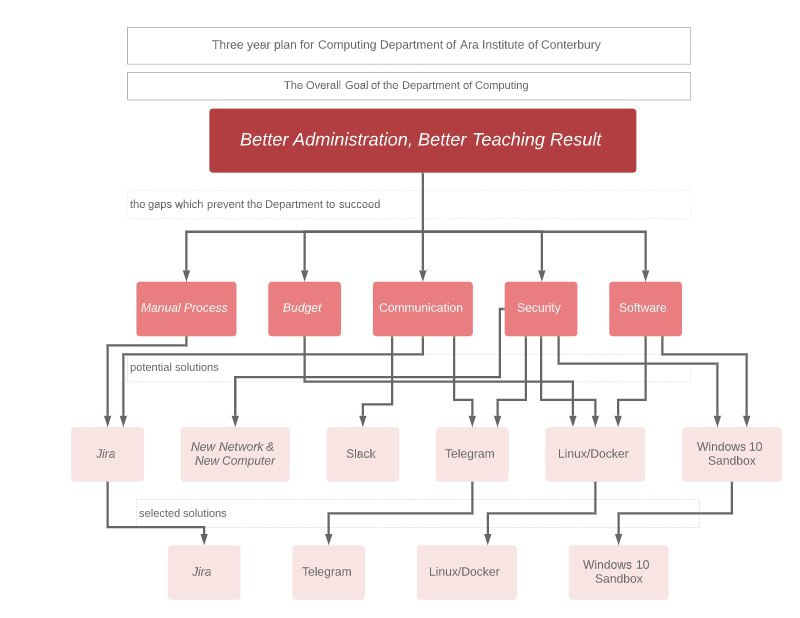
\includegraphics{hierarchy.jpg}
}
\label{img:hier}
\end{figure}
% In this section, we gather the findings of two phases of research and seek to invent a general tool for partitioners to evaluate how possible a IT project is going to succeed.


% \subsection{Summary of Findings}
% There are 21 solutions for control, 11 for people, 7 for process and 5 for structure in both phases. The same primary themes(control, people, process, structure) are used for tagging the gaps and solutions in both phases, which indicates that there is a similarity among the articles. To further investigate the agreement and the difference between the findings, we use mathematical approaches to investigate the agreement of the findings in both phases.

% \subsubsection{Average and Standard Deviation}
% In Phase 1, the average global influence score is 3.6 and the standard deviation is 2.17. In Phase 2, they are 2.66 and 1.37. It suggests the proposals in Phase 1 has a more general influence on how to make IT deployment project successful. However, standard deviation values indicate the influence of power in Phase 1 varies more than that of Phase 2.
% \subsubsection{Pie Chart by Primary Themes}
% To further our analysis on how primary themes(control, process, people and structure) distribute in both Phase 1 and Phase 2, we draw a pie chart to show the proportion.

% \begin{figure}[!ht]
% \centering
% \begin{minipage}{.5\textwidth}
%   \centering
%   %\includegraphics[width=.5\linewidth]{pie_chart_p1.png}
%   \includegraphics[height=10em]{pie_chart_p1.png}
%   \captionof{figure}{Primary Themes in Phase 1}
%   \label{pie:1}
% \end{minipage}%
% \begin{minipage}{.5\textwidth}
%   \centering
%   %\includegraphics[width=.5\linewidth]{pie_chart_p2.png}
%   \includegraphics[height=10em]{pie_chart_p2.png}
%   \captionof{figure}{Primary Themes in Phase 2}
%   \label{pie:2}
% \end{minipage}
% \end{figure}

% From Figure \ref{pie:1} and Figure \ref{pie:2}, we can conclude that the theme of control is the dominant theme of solutions followed by the theme of people, which the data of both phases agree to yield. However, there is a subtle difference in the less influential themes of process and structure. Phase 1 puts more emphasis on the structure while Phase 2 puts that on the process.

% With the mathematical analysis, we can conclude that the findings of both Phase 1 and Phase 2 are in some agreement in terms of primary themes, the values of solutions; and that we can proceed to create an evaluation tool.

% \subsection{Evaluation Tool}

% \subsubsection{The Tool}

% For each primary themes, we carry out a qualitative analysis again to mark when the solution is recommended to be used. Regarding control, we find those solutions can be divided into 3 categories, which is planning, implementation, and cooperation with vendors. Concerning people, there are two categories, which is working with people inside the same organization,  and working with people outside the organization. As for the process factor, those solutions are involved in designing the project in and implementing the project. Regarding structure,  there are two categories, which is working with people inside the organization, and working with people outside the organization.

% We populate the solutions into the predefined 2-level hierarchical structure as in section \ref{section:tool}, the evaluation tool we propose is created as in Figure \ref{table:tool}.

% \begin{figure}[ht]
% \centering
% \caption{Mark Sheet for Evaluation}
% \resizebox{\columnwidth}{!}{%
% \includegraphics{tool.png}
% }
% \label{table:tool}
% \end{figure}
% \subsubsection{Usage of the Tool}

% When a partitioner uses our evaluation tool, the partitioner should rate out of 10 for each criteria, then calculate the goal by the following formula.
% $$
% score = rate \div 10 \times weight
% $$
% And the total score is calculated by
% $$
% Total = score_1 + score_2 + score_3 + \ldots + score_{n-1} + score_n
% $$
% A higher total score indicates the higher possibility of success.

%!TEX root = ../assignment2.tex

\section{Summary}

% In this article, we have discussed what makes IT deployment successful by the following procedure of introduction, methodology, findings of Phase 1, findings of Phase 2, outcome, conclusion, summary and reflections. 


% In introduction, a brief information has been given, stating what we are investigating and what result we will produce. 3 keywords of project management, change management and risk management have been introduced to fund our further research. The methodology have covered how we do our qualitative analysis, how the evaluation is designed and how to make our own evaluation tool. A subsequent findings of Phase 1 has presented with the primary themes we identified with some samples of our findings in each theme. They are control, people, process and structure. We have also done the evaluation process for the proposals to select the solutions in this phase. As a result, 21 solutions have been selected. The findings of Phase 2 is structurally similar to the previous section, but with 10 case studies. The same primary themes have been identified as well. We have provided some samples in each primary themes as well. With the same evaluation process, we have selected 21 solutions in evaluation process. In outcome, we have analyzed the findings of both phases and found that there is a certain degree of agreement in the findings of the two phases. We have proceed to create our own evaluation tool with the predefined method in the methodology, which has produced a mark sheet for practitioners to use. In conclusion, we look back what we have done section by section.


%%%%%%%%%%%%%%%%%
% 参考文献
%%%%%%%%%%%%%%%%%
% \printbibliography
\end{document}
